\documentclass[problem]{mcs}

\begin{pcomments}
  \pcomment{CP_numbered_trees}
  \pcomment{from: S09.cp9r, edited by ARM 11/3/09}
%  \pcomment{has a pset problem associated with it}
\end{pcomments}

\pkeywords{
  counting
  bijections
  trees
  numbered_trees
}

%%%%%%%%%%%%%%%%%%%%%%%%%%%%%%%%%%%%%%%%%%%%%%%%%%%%%%%%%%%%%%%%%%%%%
% Problem starts here
%%%%%%%%%%%%%%%%%%%%%%%%%%%%%%%%%%%%%%%%%%%%%%%%%%%%%%%%%%%%%%%%%%%%%

\hyperdef{numbered}{trees}{\begin{problem}}
An $n$-vertex \term{numbered tree} is a tree whose vertex set is
$\set{1,2,\dots,n}$ for some $n > 2$.  We define the \emph{code} of
the numbered tree to be a sequence of $n-2$ integers from 1 to $n$
obtained by the following recursive process:

\textbox{If there are more than two vertices left, write down the
  \emph{father} of the largest leaf\footnote{The necessarily unique
    node adjacent to a leaf is called its \term{father}.}, delete this
  \emph{leaf}, and continue this process on the resulting smaller
  tree.

  If there are only two vertices left, then stop ---the code is complete.
}

For example, the codes of a couple of numbered trees are shown in 
the Figure~\ref{codetrees}.

\begin{figure}[htb]
\begin{center}
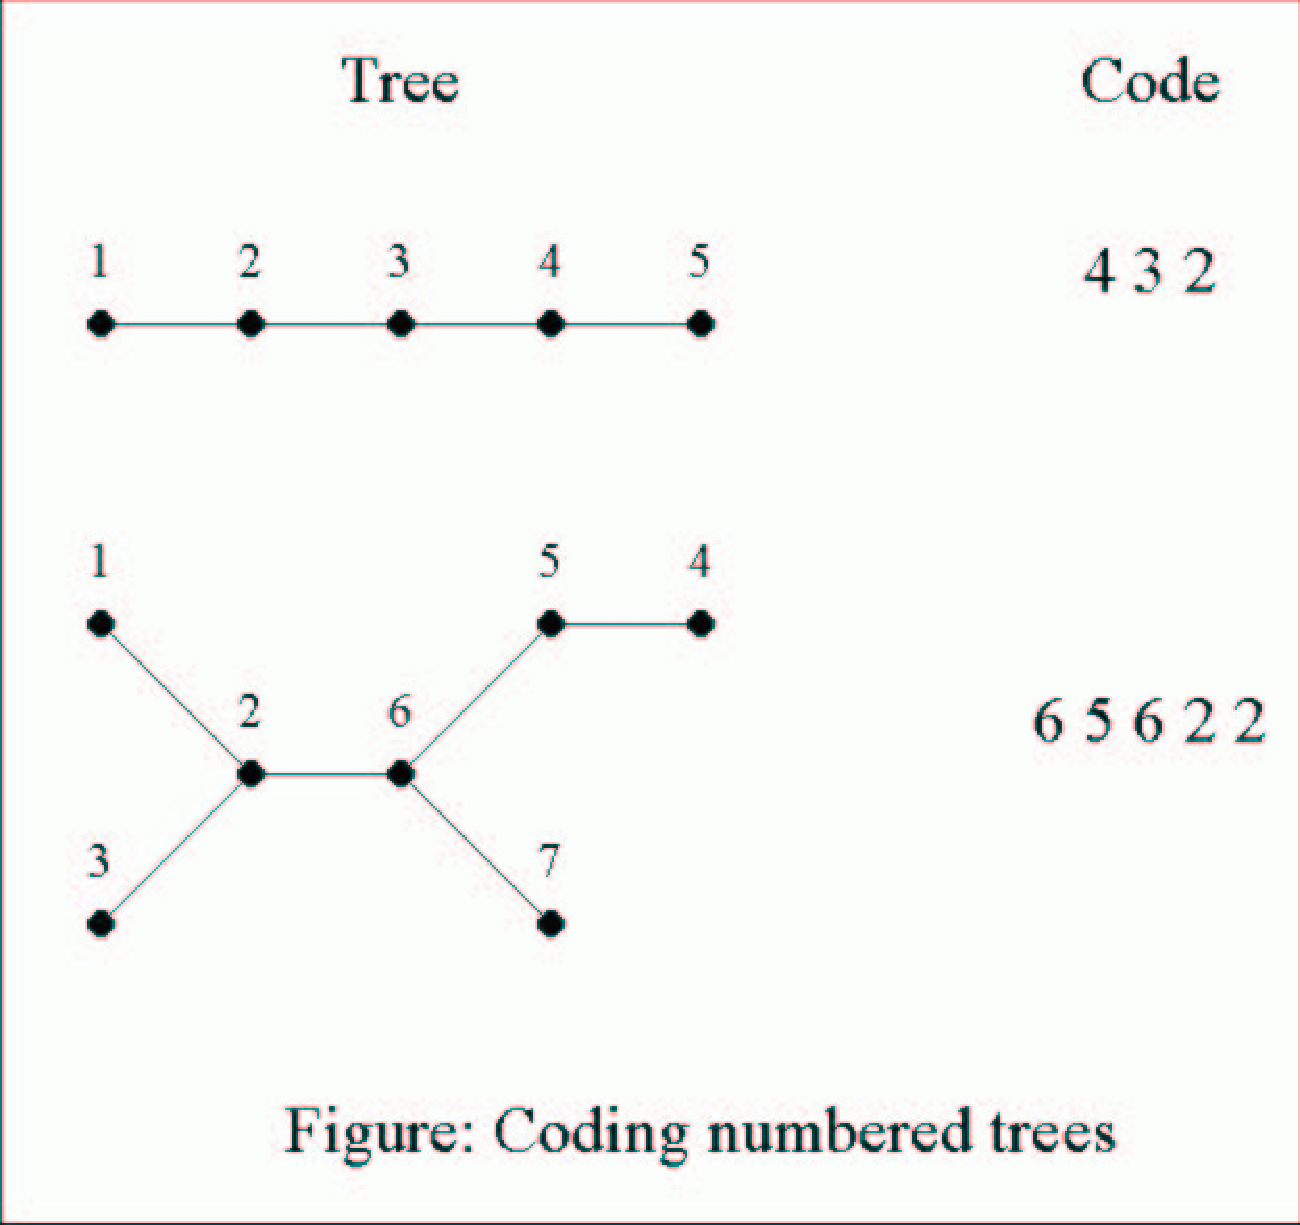
\includegraphics[width=4in]{n-2}
\end{center}
\caption{}
\label{codetrees}
\end{figure}

\bparts

\ppart Describe a procedure for reconstructing a numbered tree from
its code.

\begin{solution}
The key observation is that, given a code of length $n-2$, the numbers
between 1 and $n$ which \emph{do not appear} in the code are precisely
the leaves of the tree.  This follows because the vertices left at the
end of the process are both leaves.  So the procedure must have
changed all the nonleaf vertices into leaves, and this implies that
all the nonleaf vertices appear in the code.

Hence, the largest missing number is a leaf attached to the
first number of the code.  The rest of the tree can now be reconstructed
by deleting the first number in the code, henceforth ignoring the largest
leaf, and proceeding recursively on the rest of the code.  (We're using
the obvious fact that what's left after deleting a leaf from a tree is
another tree.)

More precisely, the reconstruction procedure applies to any finite tree
whose vertex set is totally ordered.  The procedure takes \emph{two}
parameters: the vertex set, $V$, and a length $\card{V}-2$ ``code''
sequence, $S$, of elements in $V$.  If $l$ is the largest element in $V$
which does not appear in $S$, and $f$ is the first element of $S$, then
the reconstructed tree is obtained by adding edge $(l,f)$ to the tree
reconstructed by calling the procedure recursively with first argument
$V-\set{l}$ and second argument equal to the code obtained by erasing the
initial $f$ from $S$.  The procedure terminates when $\card{V}=2$,
returning the edge between the two numbers in $V$.

\end{solution}

\ppart Conclude there is a bijection between the $n$-vertex numbered
trees and $\set{1,\dots,n}^{n-2}$, and state how many $n$-vertex
numbered trees there are.

\begin{solution}
There are exactly as many $n$-vertex numbered trees as the
number of possible code words, that is, the number of length $n-2$
sequences of integers between 1 and $n$.  So there are $n^{n-2}$ numbered
trees.
  
The reason is that the map from trees to codes is a bijection.  To see
this, note that the tree reconstruction procedure finds \emph{the only
  possible tree} with that code.  So there can't be two trees with the
same code, that is, the map from a tree to its code is an injection.  But
since the reconstruction procedure finds a tree for every possible
codeword, the map from trees to codes is also a surjection.
\end{solution}

\eparts
\end{problem} 

%%%%%%%%%%%%%%%%%%%%%%%%%%%%%%%%%%%%%%%%%%%%%%%%%%%%%%%%%%%%%%%%%%%%%
% Problem ends here
%%%%%%%%%%%%%%%%%%%%%%%%%%%%%%%%%%%%%%%%%%%%%%%%%%%%%%%%%%%%%%%%%%%%%
